\section{Сравнение одноэлектронных спектров при временном и амплитудном считывании}\label{sec:secNxVsPadiwa}

Как отмечено в секции~\ref{sec:secMapmt}, у МА~ФЭУ H12700 имеются особенности, которые могут оказать влияние на эффективность регистрации единичных фотоэлектронов и вероятность возникновения ложных хитов. Для прояснения этих особенностей были выполнены измерения амплитудных распределений с помощью многоканальной платы на основе микросхемы n-XYTER, см.~описание лабораторного стенда в секции~\ref{sec:secLabSetup}. Далее, результаты амплитудных измерений были сопоставлены с данными, полученными с помощью платы PADIWA.

Амплитудные измерения с низким порогом продемонстрировали наличие заметного пика в малых амплитудах в спектре событий, скоррелированных с источником света. Также были выполнены специальные измерения с маской, открывающей только два разнесенных друг от друга на 2.5~см. пикселя. Эти измерения позволили установить, что событие с малой амплитудой в одном из каналов имеет место тогда, когда в другом канале, находящемся в том же ряду динодной системы, был зарегистрирован фотоэлектрон с достаточно большой амплитудой. Таким образом, для каналов с низкими шумами амплитудный спектр одноэлектронных сигналов выглядит как на \figref{fig:PeculiarSpectrum}.

\begin{figure}[H]
\centering
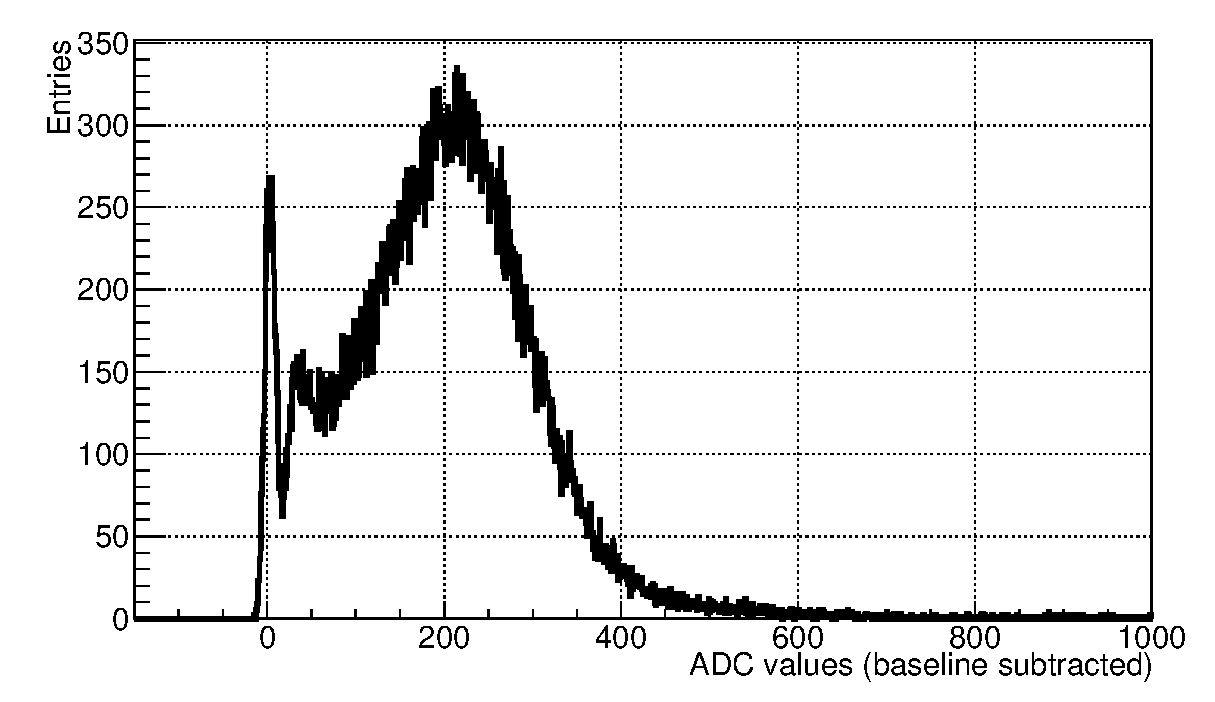
\includegraphics[width=1.0\textwidth]{pictures/30_PeculiarSpectrum.eps}
\caption{Пример измеренного одноэлектронного спектра, имеющий особую форму, характерную для МА~ФЭУ H12700.}
\label{fig:PeculiarSpectrum}
\end{figure}

Пик вблизи нуля соответствует наводке, возникающей в каналах, расположенных в одном ряду с тем, где зарегистрирован одноэлектронный сигнал. Двугорбое распределение справа соответствует настоящим одноэлектронным сигналам. Причем левый пик связан с описанными в секции~\ref{sec:secMapmt} событиями, когда электронная лавина или её часть отклоняется от оптимального пути от динода к диноду. Отметим, что в большинстве каналов уровень шумов оказывается слишком высоким для отделения низкоамплитудного пика, связанного с наводкой, от одноэлектронного сигнала. Таким образом, попытка получить максимальную эффективность регистрации за счет снижения порога приводит к возрастанию паразитных хитов, локализованных не в тех пикселях, где родился фотоэлектрон. Для снижения числа паразитных хитов мы ставили порог регистрации в ложбине между низко- и высоко-амплитудными частями одноэлектронного спектра. Поскольку формы одноэлектронных спектров во всех каналах подобны, анализ формы спектра на \figref{fig:PeculiarSpectrum} позволяет заключить, что выбранный нами порог приводит к потере~12~\% одноэлектронных импульсов.

% Пунктуация в следующем предложении.
Одно из отличий канала считывания в плате PADIWA --- это значительно более быстрая, чем в n-XYTER аналоговая часть. Если в n-XYTER осуществляется формирование со временем интегрирования 190~нс, то в PADIWA происходит лишь подавление частот выше 100~МГц, что соответствует характерному времени нарастания сигнала несколько наносекунд. Такое отличие приводит к возрастанию роли быстрых шумов и наводок при регистрации сигналов с помощью PADIWA.

Информация о форме одноэлектронного спектра при считывании с помощью канала на основе плат PADIWA и TRB~v3 может быть получена в виде зависимости от порога регистрации скорости счёта в событиях, построенных вблизи триггера светового импульса. Такие данные могут быть получены из анализа потока даных, набранных при различных значениях порога. Использование счетчика зарегистрированых фронтов, реализованного непосредственно в ВЦП и упомянутого в секции~\ref{sec:secModule}, позволяет получить аналогичную зависимость без отбора вокруг триггера, но позволяет достичь максимальных частот, достаточных для локализации базовой линии. На \figref{fig:TDCscalerScan} показана зависимость частоты триггеров от порога регистрации. Плечо слева соответствует одноэлектронному спектру, более подробно исследованному ниже, а быстровозрастающие границы вокруг вертикальной штриховой линии ограничивают локализацию базовой линии. Точность локализации базовой линии мы оцениваем как $ \pm $~200 отсчетов по шкале, использованной на \figref{fig:TDCscalerScan} и \figref{fig:Blackboard}B,D.

%\begin{figure}[H]
%\includegraphics[width=1.0\textwidth]{pictures/Thr_scan_flat.eps}
%\caption{Зависимость скорости счёта в одном канале от порога дискриминатора. Красная линия --- результат аппроксимации многочленом 7 степени.}
%\label{fig:ThrScan}
%\end{figure}

%\begin{figure}[H]
%\includegraphics[width=1.0\textwidth]{pictures/Derivative_flat.eps}
%\caption{Аналитическая производная аппроксимирующей функции --- аналог одноэлектронного спектра.}
%\label{fig:ThrScanDeriv}
%\end{figure}

\begin{figure}[H]
\centering
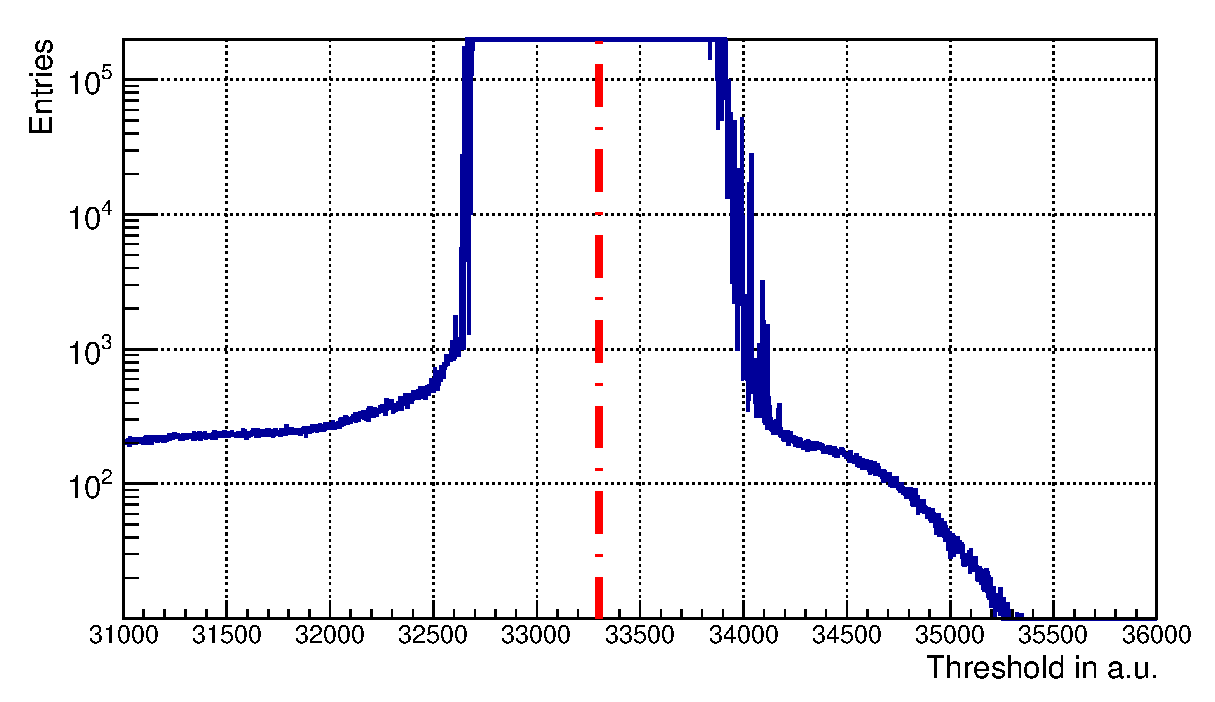
\includegraphics[width=1.0\textwidth]{pictures/31_cMean12.eps}
\caption{Скан по порогам дискриминатора в диапазоне, включающем базовую линию, изображённую штрихпунктирной линией.}
\label{fig:TDCscalerScan}
\end{figure}

Установлено, что результаты измерения частоты отсчетов, полученные с помощью счетчика и из анализа потока данных, совпадают между собой при условии, что система сбора и передачи данных справляется с передачей потока сообщений с временными отметками.

Интересно сравнить зависимость скорости счёта от порога при использовании двух систем считывания и одинаковых условиях засветки. Результаты такого сравнения для одного из типичных каналов показаны на \figref{fig:Blackboard}. В случае n-XYTER в таком сравнении может быть использован интеграл одноэлектронного спектра, показанный на \figref{fig:Blackboard}(c). Соответственно, производная указанной зависимости может быть сопоставлена с одноэлектронным спектром, показанным на \figref{fig:Blackboard}(a). Сплошная линия на \figref{fig:Blackboard}(b) получена дифференцированием кривой, показанной красным цветом на \figref{fig:Blackboard}(d) и полученной подгонкой измеренной зависимости полиномом 7-й степени. Отметим, что мы оцениваем равенство световых потоков как $ \pm $5\%. Видно, что скорости счёта в области ложбины и максимума одноэлектронного спектра приблизительно совпадают. Амплитуды, соответствующие максимуму и ложбине соответственно, относятся как 2.6 в обоих случаях. При этом, в случае PADIWA наблюдается, с одной стороны более явно выраженная ложбина, а с другой --- избыток счёта в малых амплитудах, что предполагает больший относительный вклад наводок и, следовательно, невозможность отделения от них низкоамплитудной части одноэлектронного спектра и нецелесообразность повышения эффективности за счёт установления порога ниже ложбины.

\begin{figure}[H]
\centering
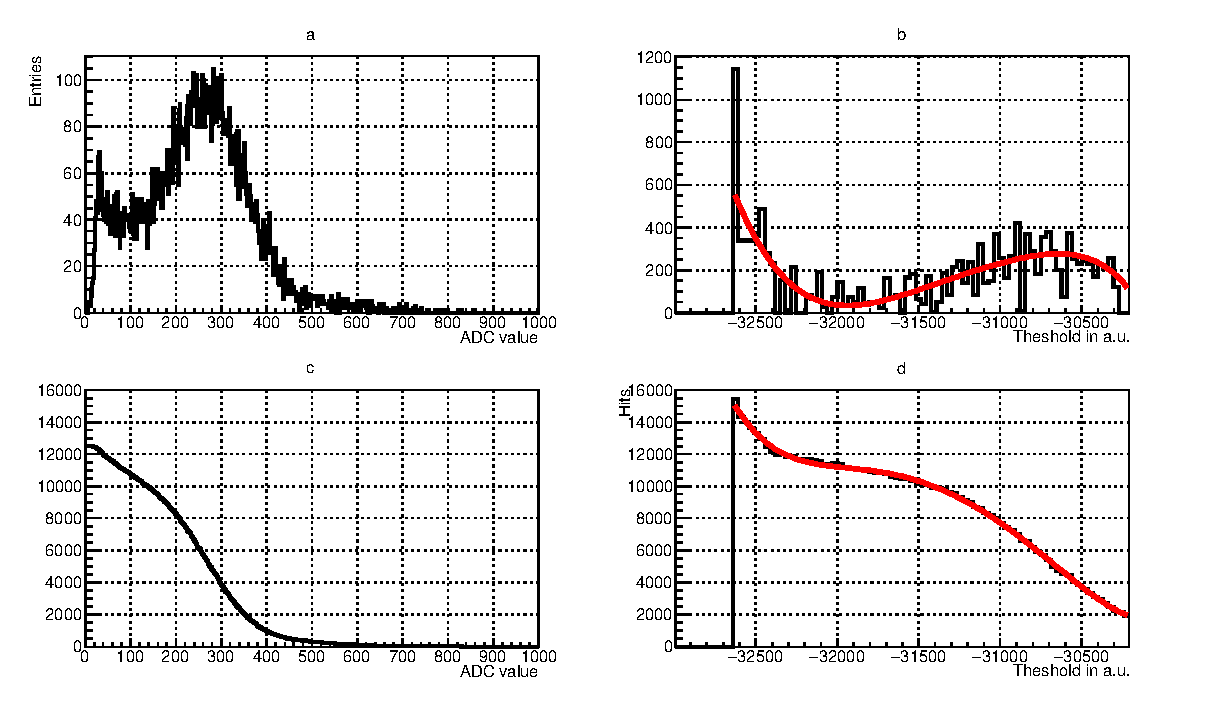
\includegraphics[width=1.0\textwidth]{pictures/32_Blackboard_4feb.eps}
\caption{Сравнение (a) одноэлектронного спектра, измеренного напрямую с помощью системы считывания на базе n-XYTER, и (b) производной скана по порогам, полученного с помощью системы считывания на базе PADIWA и TRB~v3; сравнение (c) интеграла одноэлектронного спектра и (d) зависимости скорости счёта от порога дискриминатора.}
\label{fig:Blackboard}
\end{figure}
